\cotefile{161-2}
\scanpage{81}
% slanted; a brace links the note to the two doubly circled entries.
\margin{Traiter ce cas avec quelques détails $\Biggl\{$}
\textcircled{\textcircled{1}} $\varprojlim$ finies, foncteurs exacts

\textcircled{\textcircled{$1'$}} $\varprojlim$ de types $d'$, foncteurs qui y commutent

\textcircled{$1''$} Catégories \inserted{pré}\uline{ordonnées} avec $\mathrm{Inf}$ finis, foncteurs qui y commutent

\textcircled{2} $\varprojlim$ finies et $\varinjlim$ finies, foncteurs exacts

\textcircled{$2^{\mathrm i}$} Prétopos (\uline{axiomes} \inserted{``finis''} des topos) foncteurs exacts

\textcircled{$2^{\mathrm{ii}}$} Catégories \uline{semi-additives}, foncteurs additifs

\textcircled{$2^{\mathrm{iii}}$} Catégories \uline{additives}, foncteurs additifs

\textcircled{$2^{(\mathrm{iv})}$} Catégories \uline{abéliennes}, foncteurs exacts

\hfill[foncteurs additifs ?]

\deleted{\textcircled{$\unsure{2^{(\mathrm v)}|2^{\mathrm{iv}}}$}}

\textcircled{3} $(\mathrm{Cat}_{d})$, ou $(d',d'')$ petits

\textcircled{4} Cat avec $\varprojlim$ finies, $\varinjlim$ filtrantes exactes, foncteurs y commutant

\textcircled{$4''$} Cat. préordonnées avec $\inf$ finis, $\sup$ quelconques, \deleted{qui y co}\inserted{et \unsure{tels que|que}}, $\inf$ distributifs pour $\sup$ quelc., fcteurs commutant aux $\inf$ finis et $\sup$ quelc.

% Curved arrow from 4' up to the position before 4''.
\figure{\begin{tikzpicture}\draw[->] (0,0) to[bend left=68] (0.18,.75);\end{tikzpicture}}
\textcircled{$4'$} $\varprojlim$ finies, $\varinjlim$ quelc., sommes disjointes universelles, $\varinjlim$ filtrantes exactes, foncteurs \inserted{exacts} commutant aux $\varinjlim$

\textcircled{\deleted{\unsure{5}}6} $\varprojlim$ et $\varinjlim$ quelc, foncteurs qui y commutent

% Curved arrow from Topos to the position before the preceding item.
\figure{\begin{tikzpicture}\draw[->] (0,0) to[bend left=68] (0.18,.75);\end{tikzpicture}}
\textcircled{\deleted{\unsure{6}}5} Topos

\textcircled{$6'$} Topos essentiels $(\simeq\widehat C$, i.e. ayant assez de pts essentiels, i.e. ayant les propriétés \inserted{d'exactitude} pour $\varinjlim$ et $\varprojlim$ de la cat. des ens)

Morphismes essentiels de topos.

Je m'attends à des ennuis \inserted{(de sortie de l'Univers)} \uline{au moins} avec \textcircled{6} et \textcircled{$6'$}
% archive sheet number: 80
\scanpage{82}
\diagram{\begin{tikzcd}[ampersand replacement=\&]
\mathrm{Th\acute e}_{\Delta}\arrow[r,shift left,"\rho"] \& \Delta\arrow[l,hook',shift left,"\sigma\ \text{2 fidèle}"]
\end{tikzcd}}
\margin{$\begin{aligned}\rho(T)&=B_T\quad\text{cat. des constructions sur }T\\&=\underline{\mathrm{Hom}}(T,\tau)\end{aligned}$}

\[
\sigma(R)=(C\longmapsto\underline{\mathrm{Hom}}(R,C))
\]
\margin{$\Biggl\{$ On suppose que $\rho(T)\in\mathrm{Ob}\,\Delta$ pour tout $T$, et que si $T\mathbin{\unsure{-|\to}}T'$, alors $\underline{\mathrm{Hom}}(\underset{\substack{\Vert\\\rho(T')}}{T'},\tau)\mathbin{\unsure{-|\to}}\underline{\mathrm{Hom}}(T,\tau)$ est une flèche de $\Delta$}

On a \(\underline{\mathrm{Hom}}(\sigma(R),T)\simeq T(R)\)
\[
\text{en particulier}\quad
\underset{\substack{\Vert\\\rho\sigma(R)}}{\underline{\mathrm{Hom}}(\sigma(R),\tau)}
 \simeq\tau(R)=R
\]
\margin{\uline{NB} $\rho$ défini en termes du 2-foncteur $\Delta\xrightarrow{\tau}(\mathrm{Cat})$ i.e. la 2-catégorie cofibrée fondamentale $\tau$ sur $\Delta$\ldots}

donc $\rho\sigma(R)\simeq R$ et $\sigma$ est 2 fidèle [qui vit dans toute 2-cat.]

\[
\deleted{\mathrm{Hom}_{\Delta}(R,\unsure{R'|R})\simeq}
\]
\diagram{\begin{tikzcd}[ampersand replacement=\&,column sep=small]
\& T(R)\arrow[dr] \& \\
\underline{\mathrm{Hom}}_{\mathrm{Th}}(\sigma(R),T)\arrow[ur,phantom,sloped,"\simeq"]\arrow[rr] \& \&
\underline{\mathrm{Hom}}_{\Delta}(\rho(T),\underset{\substack{\Vert\\\rho\sigma(R)}}{R})=(\sigma(\rho(T)))(R)
\end{tikzcd}}
\margin{$T(R)\times\underbrace{\rho(T)\to R}_{\Delta}$}
\inserted{est-ce une équivalence ? C'est vrai pour tt $R$ ssi $T$ 2-repr. par $\rho(T)$}

\[
\deleted{\sigma\rho(T)\xrightarrow{\text{can à isom unique près}}T}
\]
\deleted{car $\underline{\mathrm{Hom}}(\sigma\rho(T),T)\simeq T(\rho(T))$, peut-on décrire un objet à isom unique près dans $T(\rho(T))$ ??}

\[
\boxed{T\longrightarrow\sigma\rho(T)}
\]

\deleted{C'est le morphisme universel de $T$ dans une théorie 2-représentable, car}
\[
\deleted{\underline{\mathrm{Hom}}(T,\sigma(R))\longrightarrow}
\]
% archive sheet number: 81
\scanpage{83}
\[
\Delta\ (\subset\mathrm{Cat}_{d})\subset\mathrm{Cat}
\]
\margin{Question des générateurs des $C\in\mathrm{Ob}\,\Delta$. On ne se soucie pas que les objets généraux de $\Delta$ en aient ; mais ceux qui définissent des théories algébriques, oui\ldots}

\textcircled{1} Pour $I$ \unsure{$\mathrm{Ob}(\mathrm{Cat})$|$\in\mathrm{Ob}(\mathrm{Cat})$}\inserted{($I$ petit ?)}, le 2-foncteur
\[
\deleted{\unsure{I}}\quad\deleted{\unsure{I\in\mathrm{Cat}}}\quad C\longrightarrow\underline{\mathrm{Hom}}_{\mathrm{Cat}}(I,C)
\]
est 2-représentable (l'objet qui le 2-représente, soit $\widetilde I$, est appelé $\Delta$-enveloppe de $C$) : $\underline{\mathrm{Hom}}_{\mathrm{Cat}}(I,C)\simeq\underline{\mathrm{Hom}}_{\Delta}(\widetilde I,C)$
(i.e. l'inclusion $\Delta\longrightarrow\mathrm{Cat}$
\deleted{\textcircled{2} Pour \unsure{$C$} \unsure{$\in$}}
admet un 2-adjoint à gauche)

$I\mathbin{\unsure{-|\to|\mapsto}}\widetilde I$ est un 2 foncteur $(\mathrm{Cat})\longrightarrow\Delta$

\textcircled{2} Pour $\deleted{\unsure{B}}J\in\mathrm{Ob}\,\Delta$ et $\Sigma\subset\mathrm{Fl}(J)$\inserted{($\Sigma$ petit)}, le 2-foncteur
\[
\begin{aligned}
 C\longmapsto\underline{\mathrm{Hom}}_{\Delta}(J,C;\Sigma)
 &=\text{ss-catégorie pleine de }\underline{\mathrm{Hom}}_{\Delta}(J,C)\\
 &\quad\text{formée des }u:J\to C\text{ tels que}\\
 &\quad u(\alpha)\text{ inv. pour tt }\alpha\in\Sigma
\end{aligned}
\]
est 2-représentable (par une catégorie notée $J\Sigma_{\Delta}^{-1}$ ou $J\Sigma^{-1}$).

\uline{Conséquence}\quad Existence de 2-limites \inserted{inductives} dans $\Delta$, pour un pseudo foncteur
\[
\begin{aligned}
 I&\longrightarrow\Delta\\
 i&\longrightarrow\deleted{\unsure{J}}A_i
\end{aligned}
\]

Soit en effet $D=\varinjlim_{i,(\mathrm{Cat})}A_i$ la 2-limite inductive dans $(\mathrm{Cat})$\inserted{, avec $A_i\xrightarrow{\alpha_i}D$ dans $(\mathrm{Cat})$}, de sorte que pour tt $C\in\mathrm{Ob}(\mathrm{Cat})$ et \unsure{à|a} fortiori $C\in\mathrm{Ob}\,\Delta$
\[
\underline{\mathrm{Hom}}_{\mathrm{Cat}}(D,C)\xrightarrow{\simeq}\varprojlim\underline{\mathrm{Hom}}_{\mathrm{Cat}}(A_i,C)
\]
donc \deleted{$\underline{\mathrm{Hom}}_{\Delta}(\unsure{D},C)$}\inserted{$\underline L(C)$} ``est'' la sous-catégorie pleine de \deleted{$\underline{\mathrm{Hom}}$} $\underline{\mathrm{Hom}}_{\mathrm{Cat}}(D,C)$ \deleted{\unsure{associée au}} (décrite comme $\varprojlim\underline{\mathrm{Hom}}_{\Delta}(A_i,C)$) des $D\xrightarrow{u}C$ \inserted{dans Cat} tels que $\forall\,i$, $u\circ\alpha_i:A_i\to C$ soit dans $\underline{\mathrm{Hom}}_{\Delta}(A_i,C)$ ; \deleted{\unsure{On}} ou encore la sous-catégorie de $\underline{\mathrm{Hom}}_{\Delta}(\widetilde D,C)$ \inserted{des $\widetilde u:\widetilde D\to C$} tels que pour tt $i$, on ait $\widetilde u\circ\widetilde\alpha_i\in\mathrm{Ob}\,\underline{\mathrm{Hom}}_{\Delta}(A_i,\unsure{c|C})$\unsure{\})|)\}}, où $\widetilde\alpha_i$ est le composé $A_i\xrightarrow{\alpha_i}D\xrightarrow{\mathrm{can}}\widetilde D$. Or la condition
% archive sheet number: 82
\scanpage{84}
$\widetilde u\circ\widetilde{\alpha_i}$ un $\Delta$-foncteur s'exprime par la condition de rendre inversibles certaines flèches $\Sigma$ \deleted{dans}\inserted{de} $\widetilde D$ [du moins si \margin{\figure{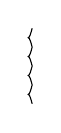
\begin{tikzpicture}\draw (0,0) sin (-.05,.12) cos (0,.24) sin (-.05,.36) cos (0,.48) sin (-.05,.60) cos (0,.72) sin (-.05,.84) cos (0,.96);\end{tikzpicture}}}on suppose que les $\Delta$-foncteurs sont définis par des prop. de commutation à certains types de $\underset{\leftrightarrow}{\lim}$ qui existent dans toutes les cat. éléments de $\Delta$]. Il n'est pas clair qu'on puisse se réduire au cas $\Sigma$ petit (si les $A_i$ \unsure{en|ne} sont petites\ldots, ce qui n'est \uline{guère} le cas que si les \unsure{p.quets|paquets|types} de diagrammes $d',d''$ par rapport auxquels on veut prendre des $\varprojlim$ et $\varinjlim$ et y commuter, sont petits) ; donc il faut alors travailler avec des sous-catégories ``génératrices'' petites, en un sens convenable\ldots.

Construction des 2-limites dans $(\mathrm{Cat})$ : elle est faite dans SGA 4 \uline{VI} en prenant la catégorie totale de la catégorie cofibrée envisagée et en rendant inversibles les morphismes cartésiens.

\medskip\hrule\medskip

``Théorie'' $T$ sur $\Delta$ : 2-catégorie cofibrée sur $\Delta$ i.e. 2-pseudofoncteur
\[
\Delta\xrightarrow{T}\mathrm{Cat}
\]
Ils forment une 2-catégorie
\[
\mathrm{Th\acute e}(\Delta)
\]
Dedans, on a
\[
\tau\in\mathrm{Ob}\,\mathrm{Th\acute e}(\Delta)\qquad \tau(C)=C
\]
On pose
\[
\underline{\mathrm{Hom}}_{\deleted{\unsure{\Delta}}}(T,\tau)=B_T\qquad
\text{catégorie \deleted{classifiante}\inserted{des constructions}}
\]
\uline{NB} Si $T$ est 2-représenté par $R\in\mathrm{Ob}\,\Delta$
\[
T(C)\simeq\underline{\mathrm{Hom}}_{\Delta}(R,C)
\]
alors on a \deleted{\unsure{Équiv|Équiv.}} pour tte théorie $T'$ sur $\Delta$
\[
\underline{\mathrm{Hom}}(T,T')\simeq T'(R)
\]
en particulier
\[
B_T=\underline{\mathrm{Hom}}(T,\tau)\simeq\tau(R)=R
\]
% archive sheet number: 83
\scanpage{85}
ce qui implique en particulier que $B_T\in\mathrm{Ob}\,\Delta$ (si $\Delta$ est défini par des propriétés d'exactitude, cela est clair, car dans $B_T=\underline{\mathrm{Hom}}(T,\tau)$ les $\underset{\unsure{\leftrightarrow|\leftarrow}}{\lim}$ de type $d',d''$ se construisent argument par argument)\unsure{;|}. Mais il y a un ``grain de sel'', c'est qu'il n'est pas clair que $B_T$ soit une $\mathcal U$-catégorie.

La description de $B_T$ qu'on a donné peut sembler brutale ; on va définir pas à pas une catégorie $B'_T$ de ``constructions explicites'' (sic) pour une \deleted{catégorie}\inserted{théorie} \uline{algébrique} $T$, quand on construit cette notion de théorie algébrique. Mais on supposera que $B'_T\in\mathrm{Ob}\,\Delta$.

\textcircled{a} Structure vide sur $I$ objets : correspond à \deleted{\unsure{$\tau$}} la ``théorie'' $\tau^I$. Elle est représentable par la $\Delta$-enveloppe \deleted{$\widetilde I$} de la catégorie discrète $I$. \deleted{Les objets de $\widetilde I$ sont sans doute obtenus} On pose $B'_{\tau^{I}}=\widetilde I$. On le justifie \inserted{(si $\Delta$ défini par ax. d'exactitude)} en \deleted{\unsure{notant}}\inserted{expliquant} qu'on peut expliciter $\widetilde I$ par lim de types $d$ à partir des objets $i$, et des axiomes d'exactitude en inversant des flèches grâce aux axiomes d'exactitudes

\[
\deleted{\unsure{\Delta\times I\quad I_{\Delta}|I\times I\quad I_{\Delta}}}
\]

\textcircled{b} Structure \unsure{déduit|déduite} d'une structure $T$ \inserted{(\deleted{avec cat. de constr. Explicite}\inserted{avec cat de constructions} $,B'_T$)} en ajoutant des axiomes : \deleted{\unsure{en joignant|en ajoutant}}\inserted{un paquet} de flèches \inserted{$\Sigma$} de $B'_T$ doivent être rendues inversibles\inserted{$B'_{T'}=B'_T\Sigma^{-1}$ (sur $\Delta$)} ;
% margin note written sideways; an arrow connects the note to the axioms.
\margin{il faut aussi prévoir les axiomes du type ``flèches rendues égales'' (en réalité, \unsure{un des|cas des|pas des} précédents si on suppose p.ex. $d'=d''=\varnothing$)}
% slanted
\margin{commentaire sur le type d'axiomes : axiomes d'iso, \inserted{ou égalités de flèches} de \deleted{\unsure{propriété}} \unsure{univers.} d'is., presque \unsure{quelconque} dans \unsure{op.} \unsure{quelques détails p.ex.} \uline{\unsure{sauf le cas exact}}. On peut rajouter des \deleted{\unsure{nouveaux}} objets de base en vrac, mais cel peut être aussi contenu dans \textcircled{d}}
\uline{NB} Si \deleted{on} $T$ est 2-repr. par \deleted{\unsure{$B'$}}$R$, \deleted{donc $B'_T\simeq R$,} alors $T'$ repr. par \deleted{\unsure{$R\Sigma^{-1}$} \unsure{soit}} $B'_{T'}$, \deleted{\unsure{alors} $R'$, car $B'_{T'}\simeq R'$.}

\inserted{Re \uline{NB} Si on a foncteurs fidèles $T\to\tau^I$, le composé $T'\to T\to\tau^I$ aussi, ($T'\to T$ pl. fid)}

\textcircled{c} Structure déduite d'une structure $T$ en ajoutant des flèches (nouvelles données) : \deleted{$\forall\,x,y\in B'_T$, ens $\unsure{H_{xy}|H_{x,y}}$ (\unsure{qui peut être vide})} \unsure{i.e.|On} $H$ un ensemble d'indices, et $H\longrightarrow\mathrm{Ob}\,B'_T\times\mathrm{Ob}\,B'_T$ \quad $h\longmapsto s(h)$, $h\longmapsto b(h)$, et on pose
\[
\begin{aligned}
T'(C)={}&\text{catégorie des objets }x\text{ de }T(C),\\
&\text{\uline{munis} d'une application }\varphi\text{ de}\\
&H\text{ dans }\mathrm{Fl}(C)\text{ telle que }\forall\,h\in H\\
&\varphi(h):s(h)(x)\longrightarrow b(h)(x)
\end{aligned}
\]
% slanted
\margin{\uline{NB} On n'admet pas la donnée de sous-objets, \deleted{\unsure{mais}} on peut avoir \deleted{des} \unsure{nouvel|nouveau} objet de base et un mono de celui-ci !}
% archive sheet number: 84
\scanpage{86}
$B'_{T'}$ est obtenu à partir de $B'_T$ en regardant les flèches $H$ -- d'où catégorie, pas néc. $\in\Delta$ -- $\deleted{\unsure{B^{0}_{T'}}}\unsure{\mathcal G|G}(B'_T,H,s,b)$ (enveloppe d'un \deleted{\unsure{catég}}\inserted{type de} diagramme) \deleted{et}, en prenant la $\Delta$'enveloppe \inserted{$B^{\prime0}_{T'}$}, et en y ``rendant inv.'' \inserted{(au sens $\Delta$)} les flèches qui expriment que le composé
\[
 B_T\xrightarrow[\substack{\text{foncteur}\\\text{can (pas}\\\text{néc. un}\\\Delta\text{-foncteur)}}]{}B^{\prime0}_{T'}
 \xrightarrow[\Delta\text{-foncteur}]{}C
\]
est un $\Delta$-foncteur.

\textcircled{\unsure{$*$}} \uline{NB} Si $T$ repr. par \deleted{$R$, $T'$ repr. par $R'$ déduit de $R=\unsure{d_R|H_R}$}\inserted{et $B'_T\simeq R$, alors $T'$ est repr par $B'$} $(=H,s_R,b_R$, où $s_R,b_R$ déduits de $s,b:H\mathbin{\unsure{-|\to}}\mathrm{Ob}\,B'_{T'}$ en comp. avec

\uline{Re NB}\quad $T'\mathbin{-}T$ fidèle, donc si on a un foncteur fidèle $T\mathbin{-}\tau^I$, le composé aussi.

\textcircled{d} \inserted{composition de structures \unsure{alg.}} Si on a des \deleted{\unsure{cat}} théories $T_\alpha$, avec $B'_{T_\alpha}$, alors la théorie $T'=\prod T_\alpha:C\mapsto\prod T_\alpha(C)$ est une structure alg.
\[
 B'_{T'}=\text{2-somme amalgamée des } B'_{T_\alpha}\text{ dans }\Delta .
\]
% slanted
\margin{\uline{petit} ens. d'indices $\alpha$}

\uline{NB} Si les $T_\alpha$ repr par les $B'_{T_\alpha}$, alors $T'$ repr. par \deleted{\unsure{le}} $B'_{T'}$.

\uline{Re NB}\quad Si $T_\alpha\mathbin{-}\tau^{I_\alpha}$ fidèl, alors $T'\mathbin{-}\tau^{I'}$ fidèl, où $I=\coprod I_\alpha$
% slanted
\margin{\uline{insuffisant}}

Si on préfère ne pas changer en cours de route des objets de base, on posera

\textcircled{$d'$} \inserted{(Composition de structures avec \deleted{\unsure{objet|objets}} bases fixées)} Si on a des théories $T_\alpha$ \deleted{[fidèles sur $\tau^I$]} $\varphi_\alpha:T_\alpha\mathbin{-}\tau^I$, alors le produit 2-fibré des $T_\alpha$ sur $\tau^I$
\[
 T'(C)=\prod_{\alpha\unsure{\,/\,|\,,\,}C^I}^{(2)}T_\alpha(C)
 \qquad\deleted{\text{(fibrés sur }\unsure{-}}
\]
\deleted{\unsure{est}} On pose $B'_{T'}=$ \deleted{\unsure{caté}} somme amalgamée des $B'_{T_\alpha}$ sur $B'_{\tau^I}=\widetilde I$.

\uline{NB} Si les $T_\alpha$ repr par les $B'_{T_\alpha}$, $T$ l'est par $B_T$.

\uline{Re NB} \deleted{\unsure{Si les}} On peut vouloir se restreindre \unsure{aux|au x} $T_\alpha\mathbin{-}\tau^{\unsure{I_\alpha|I}}$ fidèles, alors $T'\to\tau^I$ est fidèle.
% archive sheet number: 85
\scanpage{87}
% archive sheet number: 86
On peut poser à l'autre extrême

\textcircled{$d''$} $\varprojlim$ de théories (sans conditions particulières) \ldots\ Il suffirait de le postuler en un cas d'indices bien ordonné\unsure{s|s.|e}\ldots

\uline{Remarque 1}\quad On ne sort à aucun moment des théories $T$ 2 représentables par $B_T$, où $B_T=R$ \deleted{\unsure{si} \unsure{eng.}}\inserted{admet une petite} \deleted{famille} \unsure{gén.}, $I\to\mathrm{Ob}\,R$, i.e. telle que $\forall C\in\mathrm{Ob}\,\Delta$, $\underline{\mathrm{Hom}}_{\Delta}(R,C)\xrightarrow[\mathrm{fidèle}]{}\deleted{\underline{\mathrm{Hom}}}C^I$

\deleted{Remarque}

\uline{Remarque 2}\quad Soit réciproquement $R\in\mathrm{Ob}\,\Delta$, avec $\Delta$-gén. $I\to\mathrm{Ob}\,R$. \deleted{On va procéder \unsure{Soit Munissons}} \deleted{$T_0$ repr par $\unsure{\tau} R_0=\widetilde I$}

$1^\circ)$ $R$ \uline{petite}. On prend $I=\mathrm{Ob}\,R$, \unsure{qui|on|ou} part de
\[
T_0=\tau^I\ ;\ B'_{T_0}=\widetilde I=R_0
\]
On prend ensuite $H=\mathrm{Fl}(R)$, qu'on envoie dans $\mathrm{Ob}\,R_0\times\mathrm{Ob}\,R_0$ par le composé
\[
 H\longrightarrow\underset{\substack{\Vert\\I\times I}}{\mathrm{Ob}\,R\times\mathrm{Ob}\,R}
 \longrightarrow\mathrm{Ob}\,R_0\times\mathrm{Ob}\,R_0
\]
d'où $\underset{\unsure{A}}{T_1},R_1$ avec $\underset{\substack{\uparrow\\ I}}{R_0}\mathbin{\unsure{-|\to}}R_1$, $T_1\xrightarrow[\deleted{\mathrm{fid}}]{}T_0$.

% slanted; brace alongside the first three stages.
\margin{$\Biggl\{$ les trois premiers pas montrent que si $J$ est petite, la théorie $C\mapsto\underline{\mathrm{Hom}}_{\mathrm{Cat}}(J,C)$ (2-représenté par $\widetilde J$) est une théorie alg.}

On exprime ensuite que la \inserted{composition des} flèches de $R$ devient la comp. des flèches de $R_1$ i.e. \deleted{l'application} ``préfoncteur'' $R\to R_1$ devient un foncteur. On trouve ainsi
\[
T_2,R_2,\qquad R_1\mathbin{-}R_2,\quad\text{où }R_2=\widetilde R
\quad(T_2(C)\simeq\mathrm{Hom}_{\mathrm{Cat}}(R,C))
\]
On exprime enfin que le foncteur $R\to R_2$ devient un $\Delta$-foncteur, \deleted{\unsure{en}} [i.e commute à certains types de lim] en écrivant que certaines flèches de $R_2$ deviennent inversibles, d'où
\[
 T_3,R_3\qquad R_3=R .
\]
% slanted
\margin{On utilise ici que les $\Delta$-foncteurs $=$ à ceux qui commutent à certains types de lim\ldots\ Sinon il faut exprimer une condition}

[\uline{NB} On a appliqué 1 fois pas a), une fois pas c), deux fois pas b), et pas du tout d)]

$2^\circ)$ $R$ quelconque, mais avec $I\mathbin{-}\mathrm{Ob}\,R$ ``générateurs''. Soit $\rho$ la sous catégor. pleine de $R$ \uline{engendrée} par $I$. On a
\[
\underline{\mathrm{Hom}}_{\Delta}(R,C)\xrightarrow{\mathrm{fid}}
\underbrace{\underline{\mathrm{Hom}}_{\mathrm{Cat}}(\rho_0,C)}_{\text{théorie alg.}}
 \simeq\underline{\mathrm{Hom}}_{\unsure{\Delta|\mathrm{Cat}}}(\widetilde\rho_0,R)
\]
% slanted; third numbered case climbs up from the lower left.
\margin{$3^\circ)$ Soit $J\xrightarrow{u}I$ une flèche \unsure{$\underline{\mathrm{Cat}}$} dans $(\mathrm{Cat})$, avec $J\in\mathrm{Ob}\,\Delta$. Alors $C\mapsto$ sous-catégorie de $\underline{\mathrm{Hom}}(I,C)$ formée des $f:I\to C$ tels que $f\circ u$ soit un $\Delta$ foncteur, est 2-représ.}
\scanpage{88}
\deleted{et par suite $\widetilde\rho$} Considérons $R_0=\widetilde\rho_0\longrightarrow R$ et les flèches qui deviennent des isom, soit $\Sigma$, \deleted{\unsure{On a donc} $\widetilde\rho\Sigma^{-1}$} Soit \deleted{\unsure{$\rho_0$}} $\rho_1=R_0\Sigma^{-1}$, \inserted{$R_1=\widetilde{\rho_1}$} Alors $C\mapsto\underline{\mathrm{Hom}}_{\mathrm{Cat}}(R_0\Sigma^{-1},C)\simeq\underline{\mathrm{Hom}}_{\Delta}(R_1,C)$ est alg. $R_1\to R$. On construit une suite transfinie de catégories $R_\alpha\in\Delta$, et de $R_\alpha\to R$ ; toutes les \inserted{théories} $\sigma(R_\alpha)$ sont \unsure{algébrique|algébriques} (le passage aux \deleted{\unsure{limites|lim}}\inserted{ordinaux limites} se fait par le critère d), ou $d'$\deleted{\unsure{)|!}} , au choix). On suppose donc

\textcircled{$4^\circ$} Soit $R\in\mathrm{Ob}\,\Delta$, et $\deleted{\unsure{J}}I\xrightarrow{u}R$ un foncteur \deleted{\unsure{fidèle}}\inserted{(dans Cat.)} tel que $\forall\,C\in\mathrm{Ob}\,\Delta$, le foncteur $\underline{\mathrm{Hom}}_\Delta(R,C)\mathbin{\unsure{-|\to}}\underline{\mathrm{Hom}}_{\Delta}(R',C)$ fidèle ($u$ est \deleted{dit}\inserted{foncteur $\Delta$-}générateur). Construisons \deleted{un}\inserted{deux 2-}syst. inductif transfini de catégories $R_\alpha\in\mathrm{Ob}\,\Delta$, \inserted{$\rho_\alpha\in\mathrm{Ob}(\mathrm{Cat})$} tel que les morphismes de transition $R_\alpha\mathbin{-}R_\beta$ sont des $\Delta$-foncteurs, et \deleted{\unsure{un morphisme|les morphismes} \unsure{fonct|foncteurs}}liés en \unsure{a|à} 2-syst. inductif dans $R$ par des $u_\alpha:R_\alpha\longrightarrow R$ \inserted{$v_\alpha:\rho_\alpha\to R$} ($u_\alpha\in\mathrm{Fl}(\Delta)$), en posant
% slanted
\margin{faut il supposer $u$ pl fidèle ??}
\[
\begin{aligned}
R_0 &=(\widetilde I,\ \deleted{\unsure{\xi}}\ u_0:\widetilde I\mathbin{-}R\text{ prolongeant }u),\ \rho_0=R_0\\
R_{\alpha+1}&\ \inserted{\mathbin{-}R}\ \text{déduit de }R_\alpha\mathbin{-}R\text{ en définissant }
\Sigma_\alpha=\text{ens des}\\
&\qquad\text{flèches \inserted{de $R_\alpha$} qui deviennent inv. dans }R.\\
R_{\alpha+1}&=\underbrace{R_\alpha\Sigma^{-1}}_{\rho_{\alpha+1}}\quad\text{(au sens de }\Delta)
\end{aligned}
\]
% slanted
\margin{\deleted{prendre} \inserted{sous-}plutôt \inserted{partout ?} $R_{\alpha+1}=$ image essentielle de $R_\alpha\Sigma^{-1}$ dans $R$ (sous-cat. pleine de $R$) ?\par $\rho_{\alpha+1}\mathbin{-}R_{\alpha+1}\mathbin{-}\rho_{\alpha+2}\mathbin{-}R_{\alpha+2}$}
\[
 R_{\varinjlim\alpha_i}=\varinjlim_{\Delta}R_{\alpha_i}.
\]
Alors pour $\alpha$ assez grand \inserted{(dans l'univers $\mathcal U$)}, on a $R_\alpha\xrightarrow{\simeq}R$.

\uline{NB} Pour un ordinal limite, on voit que $\rho_\alpha\mathbin{-}R$ est conservatif \unsure{!!|?}. Si les $\Delta$-foncteurs \deleted{envisagés sont par} \deleted{\unsure{soit un}} commutent aux noyaux (\unsure{E|et|\ensuremath{=}} \unsure{que x|ceux|quot.} \unsure{et|ci} existent) ou conoyaux (itou), cel implique que les foncteurs $R_\alpha$ sont \deleted{pl. fidèl} \uline{fidèles}, donc les $R_\alpha$ sont des sous-catégories. Pour tt cardinal $c$, si $\alpha$ est plus élevé que $c$, $R_\alpha$ est stable sous les limites de types $\delta'\in d'$ ou $\delta''\in d'$ pour $\mathrm{card}(\delta'),\mathrm{card}(\delta'')\leq c$. Donc si $d'$ et $d''$ sont \unsure{petits|\deleted{petits}}
% slanted
\margin{avec le choix \unsure{primo|prim.} proposé on voit qu'on aura \deleted{des} \inserted{pour $\alpha$ \unsure{ind.} lim.} foncteurs pl fidèles $\rho_\alpha\subset R$, la question est si $R$ est égal à $\rho_\alpha$ pour $\alpha$ assez grand\ldots}
% archive sheet number: 87
\scanpage{90}
$\lambda$ ens de diagrammes finis

$R\in(\mathrm{Cat})_{\lambda}$ \deleted{\unsure{$R$} catégorie}

\[
\Sigma=R^\circ,\quad S=\underline{\mathrm{Hom}}_{\unsure{\lambda|\to}}(R,(\mathrm{Ens}))\subset\widehat{\Sigma}
\qquad\Sigma\subset S\subset\widehat{R^\circ}=\widehat\Sigma
\]

a) $S$ admet des $\varinjlim$ quelconques

b) $S$ est ``engendré'' par ses objets ``de \deleted{type}\inserted{prés} finie'' [objets $X$ tels que $\mathrm{Hom}(X,-)$ commute aux $\varinjlim$ \uline{filtrantes}] i.e. si $S_0$ est la ss-catégorie pl de $S$ formée de ces objets, alors
\[
 S_{\unsure{\mathrm{can}|{}}}\longrightarrow\widehat{S_0}
\]
\margin{[commute aux $\varprojlim$ quelc. et aux $\varinjlim$ filtrantes]}
est conservatif [ou $\overline{\mathrm m}$ pl. fidèle ? \inserted{ou fidèle}]

c) $\Sigma\subset S_0$ et $\Sigma$ engendre $S_0$ par $\varinjlim$ finies (resp. engendre $S$ par $\varinjlim$ quelc)

d) Plus précisément, $S_0$ est la catégorie stable par $\varprojlim$ finies \uline{enveloppante} de la $\underset{\leftarrow}{\lambda}$-catégorie \deleted{\unsure{S|\Sigma}}$\Sigma$, et $S$ est la $\varinjlim$-catégorie enveloppante de la $\varinjlim_{\unsure{0|\circ}}$-catégorie $S_0$.

Q. Relation avec ``analyseurs'' de \unsure{Lazard|Lazare}.
% archive sheet number: 89
\scanpage{91}
\uline{Dictionnaire pour $\lambda$ quelc.} $[=(\lambda_1,\lambda_2)]$

\diagram{\small\begin{tabular}{@{}p{.46\linewidth}|p{.46\linewidth}@{}}
$\lambda$-\deleted{\unsure{structures|théories}}\inserted{type}
& $\lambda$-catégorie \deleted{avec}\inserted{admettant} (petite) famille $\lambda$-génératrice\\
Morphisme de \deleted{structures}\inserted{types} $T'_\lambda\to T''_\lambda$
& $\lambda$-foncteurs $R^{\unsure{\prime\prime|\xi|\sharp}}\mathbin{-} R$\\
Morphisme pleinement fidèle \deleted{\unsure{(sous-théorie pleine)}}
& $\lambda$-foncteur de localisation $R^{\prime\prime}\mathbin{-}R'$ (p.r. à un ens de flèches) \deleted{\unsure{telles}}\\
Sous-théorie pleine $T'_\lambda\subset T_\lambda^{\unsure{\prime\prime|{}}}$
& Ens \deleted{\unsure{pas}} de flèches de $R^{\prime\prime}$ stable par composition, et par $\lambda$-limites\\
Morphisme fidèle $T'_\lambda\to T_\lambda$ [``structure plus riche'']
& $\lambda$ foncteur $f:R\to R'$ tel que $f$ $\lambda$-engendre $R'$ (\unsure{préciser|à préciser|épimorphisme ?})\\
$\lambda$-\deleted{\unsure{théorie|structures}}\inserted{structure} avec \deleted{\unsure{ens}}\inserted{famille d'objets} de base \deleted{\unsure{assurée}} $(E_i)_{i\in I}$
& $\lambda$-catégorie \inserted{$R$} avec famille d'objets $I\longrightarrow\mathrm{Ob}\,R$ qui $\lambda$-engendre $R$\\
$\varprojlim$ de $\lambda$-\deleted{\unsure{théories}}\inserted{types}
& $\varinjlim^{(\lambda)}$ de $\lambda$-catégories
\end{tabular}}

Dictionnaire \inserted{multiple} pour $\lambda=(\lambda_1,\varnothing)$

\diagram{\scriptsize\setlength{\tabcolsep}{1pt}\begin{tabular}{@{}p{.15\linewidth}|p{.20\linewidth}|p{.18\linewidth}|p{.26\linewidth}|p{.16\linewidth}@{}}
$\lambda$-type $T_\lambda$
& $\lambda$-catégorie $R$ \deleted{\unsure{avec}}\inserted{admettant} petite famille $\lambda$-génératrice
& $S\ (=R^\circ)$ $\lambda^\circ$-catégorie admettant petite famille $\lambda$-gén
& Catégorie $\mathscr C$ avec $\varinjlim$ filtrantes (et $\varprojlim$ quelc) \uline{munie} d'une sous-catégorie \deleted{\unsure{gén}}\inserted{génératrice} (pour \uline{fonct. égaux}) stable par $\lambda^\circ$ \deleted{lim} \inserted{sur \unsure{le petit}} limites formée d'objets \inserted{$A$} de prés finie (i.e. $\mathrm{Hom}(A,-)$ commute aux $\varinjlim$ filtrantes
& \deleted{\unsure{Topos $B$} \illegible{3}} Topos $B$ ayant assez de pts essentiels, et dont la cat. des pts ess. est stable par $\lambda$-lim\\[.7ex]
$T_\lambda(C)=\underline{\mathrm{Hom}}_\lambda(R,C)$ $=\underline{\mathrm{Hom}}_\lambda(S^\circ,C)$ $=\deleted{\unsure{\underline{\mathrm{Hom}}_{\varprojlim}(\mathscr C^\circ,C)|\underline{\mathrm{Hom}}(S,C)}}$ (si $C$ admet $\varprojlim$ quelc)
& $\sim$\par $R=\inserted{\unsure{\underline{\mathrm{Const}}_\lambda|\mathrm{Cat}}}\deleted{\unsure{(\mathrm{id},\mathrm{id})\text{ de }T}}S^\circ=\underline{\mathrm{Ptess}}(B)$ $=$ \uline{Objets} \inserted{ponctuels,} i.e. \unsure{rep. cov.} un \unsure{véritable|topos} $B$
& $\sim$\par $S\deleted{\unsure{=}}R^\circ:\underline{\mathrm{Fibess}}(B)=s$
& $\mathscr C=\overline{\underline{\mathrm{Hom}}_{\lambda}}(R,\mathrm{Ens})=T(\mathrm{Ens})$ $\left\{=\underline{\mathrm{Hom}}_{\lambda^\circ}(S^\circ,\mathrm{Ens})\right.$ ($=\mathrm{Ind}(S)$ si $\lambda_1=$ tous les \inserted{diagrammes finis}) $\mathscr C=\underline{\mathrm{Pt}}(B)^\circ$ \par $\cup\hspace{1.4em}\cup$\par $S=\underline{\mathrm{Ptess}}(B)^\circ$
& $\sim$\par $B=\widehat R=\underline{\mathrm{Hom}}(S,\mathrm{Ens})$ \deleted{$\unsure{\underline{\mathrm{Hom}}(C,\mathrm{Ens})}$} ($=\underline{\mathrm{Hom}}_{\unsure{\mathrm{fib}|\varprojlim|{}}}(\mathscr C,\mathrm{Ens})$ si $\lambda_1=$ ts les diag finis,\\
\multicolumn{2}{@{}p{.35\linewidth}|}{$=$ sous-catégorie pleine de $\underline{\mathrm{Hom}}(C^\circ,\mathscr C)$ formée des foncteurs $u:C^\circ\mathbin{-}\mathscr C$ dont les composés avec les $\mathrm{Hom}(X,-)$, $X\in\mathrm{Ob}\,S$, sont représentables $=\underline{\mathrm{Homtop}}(C,B)^\circ$ (si $C$ est un topos}
& & \multicolumn{2}{p{.43\linewidth}@{}}{(et \unsure{admet|plutôt} les diagrammes filtrants\ldots) $B=$ topos classifiant pour $T$}\\ \hline
morphisme $T'\mathbin{-}T$
& $\lambda$-foncteur $R^{\prime\prime}\mathbin{-}R'$ \par \ldots
& $\lambda^\circ$-foncteur $S\mathbin{-}S'$ \par \ldots
& foncteur $\mathscr C'^{\unsure{\xi|\prime|\sharp}}\to\mathscr C$ \deleted{\unsure{équiv.}} commutant aux $\varinjlim$ \unsure{quelc.} \deleted{\unsure{se place} \unsure{et commute} \unsure{à} \illegible{4} \unsure{présentations} \unsure{sont}} $\varprojlim$ quelconques (donc (?), ayant un adjoint à g.), dont l'adjoint envoie $S$ dans $S'$ ou : foncteur $\mathscr C\mathbin{-}\mathscr C'$ commutant aux $\varinjlim$ quelc et envoyant $S$ dans $S'$
& Morphismes de topos $B'\xrightarrow{f}B^{\unsure{\xi|\prime|{}}}$ tel que $f^\ast$ transforme \deleted{\unsure{objets}} ponctuels en objets ponctuels \deleted{\unsure{essentiels} \illegible{2}} \par \ldots
\end{tabular}}
% archive sheet number: 90
\scanpage{92}
\diagram{\scriptsize\setlength{\tabcolsep}{1pt}\begin{tabular}{@{}p{.16\linewidth}|p{.13\linewidth}|p{.16\linewidth}|p{.29\linewidth}|p{.20\linewidth}@{}}\hline
morphisme pl. fidèle $T'\mathbin{-}T$
& $\lambda$ foncteur de localisation $R^{\unsure{\prime\prime|\xi|\sharp}}\mathbin{-}R'$
& $\lambda^\circ$-foncteur de localisation $S\mathbin{-}S'$
& foncteur $\mathscr C'\to\mathscr C$\ldots\ \uline{pl. fidèle} (ou foncteur $\mathscr C\mathbin{-}\mathscr C'$\ldots\ de \uline{localisation})
& Morphisme de topos $B'\xrightarrow{f}B$\ldots\ qui est un \uline{plongement} i.e. $f_\ast:B'\mathbin{-}B$ pl. fid.\\ \hline
sous-théorie pleine de $T_\lambda$
& Ens de flèches $M$ de $R$ stable par comp. et par $\underset{\leftrightarrow}{\lim}$ type \unsure{$\lambda$}
& Ens de flèches $M'$ de $S'$ stable par comp. et par lim type $\lambda^\circ$
& Sous-catégorie pleine, \deleted{stable}\inserted{\unsure{(eng.}} par limites projectives, \unsure{petites|petites,} \unsure{sommes)} qui est \unsure{dite|décrite|telle} par $\mathrm{Ob}\,\mathscr C'=$ \deleted{\unsure{ens}} des objets $X$ de $\mathscr C$ tels que pour tt $u\in\deleted{\unsure{\mathrm{Fl}(S)}}S'$, avec $\mathrm{Hom}(u,\deleted{\unsure{Y|X}}Y)$ bij. pour tout $Y\in\mathrm{Ob}\,\mathscr C'$, on ait $\mathrm{Hom}(u,X)$ bijectif
& Sous-topos $B'$ de $B$ tel que, si $\deleted{f'}\deleted{B'} B'$ est le plongemt, $f^\ast$ transforme objets ponctuels en objets ponctuels [\deleted{\unsure{ceci}} déduit par localisation de $B$ par rapport à un ens de flèches de $\underset{\substack{\searrow\\\text{objets ponctuels}}}{R}\subset B$\\ \hline
\deleted{foncteur}\inserted{morphisme} fidèle de théories $T'\mathbin{-}T$
& $R\mathbin{-}R'$ $\lambda$-engendre $R'$
& $S\mathbin{-}S'$ $\lambda$-engendre $S'$
& $\mathscr C'\to\mathscr C$ fidèle (2-fid ??) ou $\mathscr C\to\mathscr C'$ induit $S\mathbin{-}S'$ qui \inserted{$\lambda$ engendre $S'$}
& $f^{\inserted{\ast}}_{\deleted{\unsure{\ast}}}:B'\mathbin{-}B^{\unsure{\xi|\prime|{}}}$ est fidèle\\ \hline
$\varprojlim$ de $\lambda$-types $(T_\lambda)_i$
& $\varinjlim$ de $\lambda$-cat. $R_i$
& $\varinjlim$ de $\lambda^\circ$-cat $S_i$
& $\varinjlim$ de \deleted{\unsure{(Dérivés}} $\varinjlim$ catégories $\mathscr C_i$ (munies de \ldots\ ; mais c'est \unsure{fîle|facile|fini} si $\lambda_1=$ tous les di$^\mathrm s$ finis
& $\varprojlim$ des topos\\ \hline
\end{tabular}}
% archive sheet number: 91
\scanpage{93}
\deleted{\unsure{Soit}} Soit $T$ l'espèce de structure ``anneau'' \inserted{(commutatif avec unité)}, $T^{\unsure{\alpha|a|\circ}}$ l'espèce de structure ``corps''. Cette dernière n'est pas définissable par $\varprojlim$ (car la catégorie des corps \inserted{(commutatifs)} n'est pas stable par $\varprojlim$, pas $\overline{\mathrm m}$ par produits finis). Leur sous-théorie pleine \inserted{de $T$} la plus petite qui soit définissable par $\varprojlim$ est \deleted{\unsure{ainsi que|admettent par} : les propriétés suivantes : sont}\inserted{définie par la sous-catégorie $\mathscr C'$ de $\mathscr C$ définie par}
\[
\begin{aligned}
C\in\mathrm{Ob}\,\mathscr C'\ \Longleftrightarrow{}&
 \ \forall\,\unsure{\mathrm{hom.}|\mathrm{Hom.}}\ A\longrightarrow B\text{ dans }(\mathrm{Ens})\text{ tel que}\\
&X=\unsure{\mathrm{Sp}|\mathrm{Spm}|h}(B)\mathbin{\unsure{-|\to}}Y=\mathrm{Sp}(A)\text{ soit bijectif : ext.}\\
&\text{résiduelles triviales, }\mathrm{Hom}_{\mathrm{ann}}(B,C)\mathbin{-}\mathrm{Hom}_{\mathrm{ann}}(A,C)\\
&\text{est bijectif.}
\end{aligned}
\]

Un tel $C$ a la propriété que $C$ est \deleted{\unsure{abs. plat}}\inserted{pseudocorps} (Spec $C$ \inserted{séparé donc} compact, \deleted{\unsure{et}} $C$ réduit \deleted{$\Longleftrightarrow$} les \deleted{anneaux locaux} anneaux locaux de $C$ des corps) -- Les $C$ sont ceux qui transforment en \unsure{isom|isom.} l'hom évident $\mathbb Z[t]\longrightarrow\mathbb Z[t,t^{-1}]\times\mathbb Z\simeq\mathbb Z[x,y]/((xy-1)x,(xy-1)y)$ transformt $t$ en $(t,0)$ resp. en $x$. La réciproque est vraie, \inserted{et connue} -- donc la catégorie \deleted{des} $\mathscr C'$ est celle des pseudocorps.

[Mais la \deleted{notion}\inserted{structure} de corps peut elle se définir par $\varprojlim$ et $\varinjlim$, du moins dans des catégories satisfaisant des conditions d'exactitude convenables ?]

Le sous-objet $A^\ast$ (des éléments inversibles) d'un \inserted{objet} anneau d'une catégorie $\unsure{\mathscr A|\mathscr C|A}$, peut-il\deleted{\unsure{le|lle}} se définir par $\varprojlim$ (ou par $\varprojlim$ et $\varinjlim$) ? Dans le premier cas, on est ramené au cas de l'objet universel dans $R=(\mathrm{Ann})^\circ$ \inserted{$=(\unsure{\mathrm{Sch\text{-}aff.}|\mathrm{Sch\ aff.}|\mathrm{Sch\,aff}}\ \deleted{\unsure{\mathrm{f.p.}}})$} qui est l'objet $\mathbb Z[t]$.
% archive sheet number: 92
\scanpage{94}
de $R$. \deleted{\unsure{Par le foncteur contravariant} \unsure{can.}}\deleted{\inserted{\unsure{identique}}} Or un ss-objet dans $R$ est un \deleted{objet \unsure{quoti}} sous-objet dans (Sch-aff), en effet $\mathbb Z[t,t^{-1}]=\underline{\mathbb Z[x,y]}/(xy-1)$. Donc O.K. \deleted{\unsure{si }\unsure{$\exists$} \unsure{lim}} avec $\varprojlim$ finies

Ceci dit, considérons pour un objet $A$ le morphisme $\deleted{\unsure{e\amalg{}}}A^\ast\longrightarrow A$, où $e$ est l'objet final. On pourra dire que $A$ (\deleted{\unsure{dans}}\inserted{anneau} dans une catégorie \deleted{quelconque}\inserted{avec $\varprojlim$ finies et $\varinjlim$ finies}) est un objet corps si ce morphisme est un isom.

Plaçons nous p.ex. dans la théorie des topos. Alors \deleted{\unsure{considér}} le topos universel \inserted{(classifiant)} pour les anneaux est $\deleted{\unsure{S}}\widehat R$ ($R\simeq\mathrm{Sch\,aff\ tf}$). L'objet anneau universel est $O=\mathbb E^1_{\mathbb Z}=\unsure{\mathrm{Spec}|\mathrm{Sp}}(\mathbb Z[t])$.

Il faut donc rendre inversible la flèche
\[
\deleted{\unsure{\mathbb Z[t]\longrightarrow B}}\qquad
\deleted{\unsure{e}}\amalg O^\ast\mathbin{\unsure{-|\to}}O
\]
(\deleted{\unsure{i.e.}}\inserted{ce n'est pas} la \unsure{transposée} (dans $R$, $D\to O$) de la flèche \inserted{(dans $\widehat R$, \uline{pas} dans $R$ !)} déjà utilisée plus haut\inserted{, car ce n'est pas une flèche dans $R$ !}) On voit que cela implique que \deleted{tte flèche $X\mathbin{-}Y$ \inserted{dans} $R$ qui est un morphisme bijectif de schémas : ext. résiduelles triviales devient un isom dans le nouveau topos classifiant $B'$. [ceci encore en remarquant que} pour tt \inserted{$X\in\widehat R$ et tt} $f\in\Gamma(X,O_X)$,
\[
 X_f\amalg V(f)\mathbin{-}X
\]
doit devenir un isom, car déduit de la situation précédente par chgt de base
\diagram{\begin{tikzcd}[ampersand replacement=\&,row sep=small]
 X\arrow[r,"f"] \& O=\mathbb E^1_{\mathbb Z}\\
 \& O^\ast\amalg e\arrow[u]
\end{tikzcd}}
] \deleted{Or la catégorie quotient de $R$ par l'inv des flèches précédentes (qui manifestement est stable par $\varprojlim$) est la catégorie des schémas \unsure{compacts|composés|complet}}
% archive sheet number: 93
\scanpage{95}
\deleted{qui sont \unsure{propres de} associés à des schémas de t.f. sur $\mathbb Z$ [ou encore la catégorie des \uline{schémas entièrt.} \uline{complets} qui sont \inserted{constr.} \unsure{de} t.f. sur $\mathbb Z$] On trouve donc que $B'=\widehat{R'}$ Ainsi, $B'$}

Comme on a une factorisation
\diagram{\begin{tikzcd}[ampersand replacement=\&]
e\amalg O^{\unsure{\times|\ast}}\arrow[r,"\varphi"]\arrow[d,maps to,"j"'] \& O\\
D\arrow[ur,hook,"i"'] \&
\end{tikzcd}}
\deleted{rendre} $\varphi$ inversible revient à rendre $D$ inversible \uline{et} $j$ inversible \inserted{(car un bimorphisme dans un topos est un isom)}. \deleted{Faisons}\inserted{rendons} d'abord les morphismes $i$ (qui sont dans $R$) inversibles, on trouve, si $R'$ est la catégorie des fractions de $R$ [\deleted{\unsure{des|i.e.}} catégorie des schémas compacts associés à des schémas de t.f. sur $\mathbb Z$], on trouve le topos $\widehat{R'}$ (classifiant pour les pseudo-corps).
% slanted
\margin{\uline{bimorphismes} ou \uline{isom.}}
% slanted
\margin{sommes de deux disjointes\ldots\ \unsure{où que|ou que}}

Il faut ensuite rendre $e\amalg O^\alpha\mathbin{-}O$ un monomorphisme i.e. \inserted{rendre} \deleted{\unsure{si}} $e\cap O^\ast$ vide, or $e\cap O^\ast\in R\mathbin{-}R'$ est le crible formé des schémas vides, représenté le foncteur \deleted{$(\varepsilon\subset\unsure{e})$\unsure{$R'$}} donné par
\[
\varepsilon(X)=\begin{cases}
\varnothing&\text{si }X\ne\varnothing\\
\{e\}&\text{si }X=\varnothing
\end{cases}
\]
\deleted{donc il faut rendre $\varnothing_{\widehat{R'}}\to\varepsilon$ un isom}

\margin{$\Big\Vert$}\uline{On trouve}\quad Si $C$ est une catégorie avec $\varprojlim$ finies et $\varinjlim$ quelconques (suffit-il qu'il y ait $\varinjlim$ finies, voire des sommes finies ?) \deleted{alors \unsure{les}} \inserted{et si} les \deleted{``\unsure{morph}'' dans $C$} bimorphismes sont des isom, alors les ``corps'' dans $C$ correspondent aux foncteurs $F:R'\to\unsure{\mathscr C|C}$ qui \deleted{commutent} sont exacts à gauche \inserted{et commutant aux sommes.}
\margin{\unsure{tgrp|trop|tgrps}}
% archive sheet number: 94
